\documentclass{birkjour}

\usepackage{amsmath}
\usepackage{amssymb}
\usepackage{amsthm}
\usepackage{graphicx}
\usepackage{float}
\usepackage{url}

\newtheorem{thm}{Theorem}[section]
 \newtheorem{cor}[thm]{Corollary}
 \newtheorem{lem}[thm]{Lemma}
 \newtheorem{prop}[thm]{Proposition}
 \theoremstyle{definition}
 \newtheorem{defn}[thm]{Definition}
 \theoremstyle{remark}
 \newtheorem{rem}[thm]{Remark}
 \newtheorem*{ex}{Example}
 \numberwithin{equation}{section}

\newcommand{\G}{\mathbb{G}}
\newcommand{\V}{\mathbb{V}}
\newcommand{\Vb}{\mathbb{\overline{V}}}
\newcommand{\W}{\mathbb{W}}
\newcommand{\R}{\mathbb{R}}
\newcommand{\B}{\mathbb{B}}

\newcommand{\Alpha}{A}
%\Omega is already defined

\newcommand{\nvao}{o}
\newcommand{\nvai}{\infty}
\newcommand{\nvaob}{\overline{o}}
\newcommand{\nvaib}{\overline{\infty}}

\newcommand{\eminus}{e_{-}}
\newcommand{\eplus}{e_{+}}
\newcommand{\eminusb}{\overline{e}_{-}}
\newcommand{\eplusb}{\overline{e}_{+}}

\begin{document}

\title{A Conformal-Like Model Of Geometric Algebra For Quadric Surfaces}

\author{Spencer T. Parkin}
\email{spencer.parkin@gmail.com}

\numberwithin{equation}{section}

\subjclass{Primary 14J70; Secondary 14J29}

\keywords{Quadric Surface, Quartic Surface, Geometric Algebra, Quadric Model, Conformal Model}

%\dedicatory{To Melinda and Naomi}

\begin{abstract}
A variation of the quadric model set forth in \cite{Parkin12} is
found in which the rigid body motions are represented by
versors applicable to any quadric surface.
Extending this variation of the original model to include
a specific form of quartic surface, we find that the versors of
the conformal model may be used to transform any such surface.
Results of a computer program implementing this new model are presented.
\end{abstract}

\maketitle

\section{Introduction}

In the original paper \cite{Parkin12}, a model for quadric surfaces was
presented based upon the ideas of projective geometry.  What was unfortunate
about this model, however, was its lack of support for the rigid body transformations.  It was
predicted in the conclusion of that paper that a better model for quadric
surfaces may exist that is more like the conformal model of geometric algebra.
The present paper details what may be such a model.  We'll find that the rigid
body transformations can be incorporated into the model by using an alternative
method of encoding the quadric form.  An extension to the quadric form
will then allow us to support the conformal transformations at the expense of
expanding our model to necessarily include a specific form of quartic surfaces.  The
new model and its extension will both use the same geometric algebra to be given as follows.

\section{The Geometric Algebra}

We begin here with a description of the structure of the geometric algebra upon
which our model will be imposed.  This
geometric algebra will contain the following vector spaces.
\begin{equation}\label{equ_vector_spaces}
\begin{array}{ll}
\mbox{Notation} & \mbox{Basis} \\
\hline
\V^e & \{e_i\}_{i=1}^n \\
\V^{\nvao} & \{\nvao\}\cup\{e_i\}_{i=1}^n \\
\V^{\nvai} & \{e_i\}_{i=1}^n\cup\{\nvai\} \\
\V & \{\nvao\}\cup\{e_i\}_{i=1}^n\cup\{\nvai\}
\end{array}
\end{equation}
The set of vectors $\{e_i\}_{i=1}^n$ forms an orthonormal set of basis
vectors for the $n$-dimensional Euclidean vector space $\V^e$, which we'll
use to represent $n$-dimensional Euclidean space.
The vectors $\nvao$ and $\nvai$ are the familiar null-vectors representing the
points at origin and infinity, respectively, taken from the conformal model of geometric algebra.
An inner-product table for these basis vectors is given as follows, where
$1\leq i<j\leq n$.
\begin{equation}
\begin{array}{c|cccc}
\cdot & \nvao & e_i & e_j & \nvai \\
\hline
\nvao & 0 & 0 & 0 & -1 \\
e_i & 0 & 1 & 0 & 0 \\
e_j & 0 & 0 & 1 & 0 \\
\nvai & -1 & 0 & 0 & 0
\end{array}
\end{equation}
We will now let $\G(\V)$ denote the Minkowski geometric algebra generated by $\V$.
For each vector space in table \eqref{equ_vector_spaces}, we will let an over-bar
above this vector space denote an identical copy of that vector space.  The vector
space $\W$ will denote the smallest vector space containing each of $\V$ and $\Vb$
as vector subspaces.  In symbols, one may write
\begin{equation}
\G(\W) = \G(\V\oplus\Vb)
\end{equation}
to illustrate the structure of $\G(\W)$ in terms of its two isomorphic Minkowski
geometric sub-algebras $\G(\V)$ and $\G(\Vb)$.

We will use over-bar notation to distinguish between vectors taken from $\V$
with vectors taken from $\Vb$.  Though not necessary, we can work exclusively
in $\G(\V)$ by defining the over-bar notation as an ismorphism between
$\G(\V)$ and $\G(\Vb)$.  Doing so, we see that for any element $E\in\G(\V)$,
we may define $\overline{E}\in\G(\Vb)$ as
\begin{equation}
\overline{E} = SES^{-1},
\end{equation}
where $S$ is the versor given by
\begin{equation}\label{equ_isomorphism_versor}
S = (1+\eminus\eminusb)(1-\eplus\eplusb)\prod_{i=1}^n(1-e_i\overline{e}_i).
\end{equation}
This definition is non-circular if we let the over-bars in equation \eqref{equ_isomorphism_versor}
be purely notation.  The vectors $\eminus$ and $\eplus$, taken from \cite{LiRockwood},
are defined as
\begin{align}
\eminus &= \frac{1}{2}\nvai + \nvao, \\
\eplus &= \frac{1}{2}\nvai - \nvao.
\end{align}
The vectors $\eminusb$ and $\eplusb$ are defined similarly in terms of $\nvaob$ and $\nvaib$.
Defined this way, realize that, like the over-bar function defined in \cite{Parkin12},
here we have the property that for any vector $v\in\V$, we have $\overline{v}=v$ and $\overline{\overline{v}}=-v$.

\section{The Form Of Quadric Surfaces In $\G(\W)$}

We now give a formal definition under which elements $E\in\G(\W)$
are representative of $n$-dimensional quadric surfaces in our present variation
of the original model.
\begin{defn}\label{def_quadric}
Referring to an element $E\in\G(\W)$ as a quadric surface, it is representative of such an $n$-dimensional surface as the set of all points $p\in\V^o$ such that
\begin{equation}\label{equ_quadric_equation}
0 = p\wedge\overline{p}\cdot E.
\end{equation}
\end{defn}
From this definition it can be seen that the general form of a quadric $E\in\G(\W)$ is given by
\begin{equation}\label{equ_quadric_form}
E = \sum_{i=1}^k a_i\overline{b}_i,
\end{equation}
where each of $\{a_i\}_{i=1}^k$ and $\{b_i\}_{i=1}^k$ is a sequence of $k$ vectors
taken from $\V^\nvai$.  To see why, realize that the form \eqref{equ_quadric_form} can
always be reduced to the form
\begin{equation}\label{equ_quadric_reduced_form}
E = \sum_{i=1}^n\sum_{j=i}^n\lambda_{ij}e_i\overline{e}_j+
\sum_{i=1}^n\lambda_i e_i\nvaib+
\lambda\nvai\nvaib,
\end{equation}
where each of $\lambda_{ij}$, $\lambda_i$, and $\lambda$ are scalars, in the
sense that this reduced form represents the same surface as that in equation \eqref{equ_quadric_form}
under Definition~\ref{def_quadric}.
We then see that this form \eqref{equ_quadric_reduced_form}, when it is
substituted into equation \eqref{equ_quadric_equation}, produces to a polynomial
equation of degree 2 in the vector components of $p-\nvao$.
Doing so with $p=\nvao+x$, where $x\in\V^e$, we get the equation
\begin{equation}\label{equ_quadric_polynomial_equation}
0 = -\sum_{i=1}^n\sum_{j=i}^n\lambda_{ij}(x\cdot e_i)(x\cdot e_j)
+\sum_{i=1}^n\lambda_i(x\cdot e_i) - \lambda,
\end{equation}
which we may recognize as the general equation of an $n$-dimensional quadric surface.

In practice, a computer program might take such a bivector of the form \eqref{equ_quadric_form}
and extract from it the coefficients of the quadric polynomial \eqref{equ_quadric_polynomial_equation} it
represents.  It could then render the surface using traditional methods, such as those used
to render the traced surfaces in Figure~\ref{fig_reflect_cylinder_in_sphere} far below.

Of course, using geometric algebra on paper, it is undesirable and unnecessary to think of
quadrics in terms of polynomial equations.  A, perhaps, better way to think of quadrics is in terms
of an element of the algebra whose decomposition
produces the parameters characterizing the quadric surface.  For example, many common
quadrics are the solution set in $\V^e$ of the equation
\begin{equation}
0 = -r^2 + (x-c)^2 + \lambda((x-c)\cdot v)^2,
\end{equation}
in the variable $x$.  (An explanation of the parameters $r$, $c$, $v$ and $\lambda$
was given in \cite{Parkin12}.)  Then, factoring out $-p\wedge\overline{p}$, we see that
the element $E\in\G(\W)$, given by
\begin{equation}\label{equ_canonical_form_of_common_quadric}
\Omega + \lambda v\overline{v}+2(c+\lambda(c\cdot v)v)\nvaib+
(c^2+\lambda (c\cdot v)^2-r^2)\nvai\nvaib
\end{equation}
is representative of this very same quadric by Definition~\ref{def_quadric},
where $\Omega$ is defined as
\begin{equation}
\Omega = \sum_{i=1}^n e_i\overline{e}_i.
\end{equation}
Canonical forms similar to \eqref{equ_canonical_form_of_common_quadric}
can be found for specific geometries, such as planes, spheres, plane-pairs,
circular cylinders, circular conical surfaces, and so on.

\section{Transformations Supported By The Model}

The main result of this section will depend upon the following lemma.
\begin{lem}\label{lma_versor_transfer}
For any versor $V\in\G(\W)$, and any four vectors $a,b,c,d\in\V$, we have
\begin{equation}
V^{-1}aV\wedge\overline{V^{-1}bV}\cdot c\wedge\overline{d} =
a\wedge\overline{b}\cdot V\overline{V}(c\wedge\overline{d})(V\overline{V})^{-1}.
\end{equation}
\end{lem}
\begin{proof}
We begin by first establishing that
\begin{align}
 & V^{-1}aV\wedge\overline{V^{-1}bV}\cdot c\wedge\overline{d} \\
&\;= -(V^{-1}aV\cdot c)(V^{-1}bV\cdot d) \\
&\;= -(a\cdot VcV^{-1})(b\cdot VdV^{-1}) \\
&\;= a\wedge\overline{b}\cdot VcV^{-1}\wedge\overline{VdV^{-1}}.
\end{align}
We now notice that
\begin{align}
& VcV^{-1} \\
=\;& V\overline{VV^{-1}}cV^{-1} \\
=\;& (-1)^m V\overline{V}c\overline{V^{-1}}V^{-1} \\
=\;& (-1)^m V\overline{V}c(V\overline{V})^{-1},
\end{align}
where $m$ is the number of vectors taken together in a geometric
product to form $V$.  We then notice that
\begin{align}
& \overline{VdV^{-1}} \\
=\;& VV^{-1}\overline{VdV^{-1}} \\
=\;& (-1)^{m^2}V\overline{V}V^{-1}\overline{dV^{-1}} \\
=\;&(-1)^{m^2+m}V\overline{Vd}V^{-1}\overline{V^{-1}} \\
=\;&(-1)^{2m^2+m}V\overline{VdV^{-1}}V^{-1} \\
=\;&(-1)^mV\overline{Vd}(V\overline{V})^{-1}.
\end{align}
It now follows that
\begin{equation}
a\wedge\overline{b}\cdot VcV^{-1}\wedge\overline{VdV^{-1}} =
a\wedge\overline{b}\cdot V\overline{V}(c\wedge\overline{d})(V\overline{V})^{-1}.
\end{equation}
\end{proof}
We're now ready to prove the main result as follows.
\begin{thm}\label{thm_quadric_transform}
Let $E\in\G(\W)$ be a bivector of the form \eqref{equ_quadric_form}.
Let $p,p'\in\V^o$ be a pair of points related by a versor $V\in\G(\V)$ by
the equation
\begin{equation}\label{equ_get_rid_ni}
p' = \nvao\cdot V^{-1}pV\wedge\nvai.
\end{equation}
Now let $E'\in\G(\W)$ be a bivector given by
\begin{equation}\label{equ_transformed_surface}
E' = V\overline{V}E(V\overline{V})^{-1}.
\end{equation}
Then, if $E'$ is of the form \eqref{equ_quadric_form}, then the
set of all points $p\in\V^\nvao$ such that
\begin{equation}\label{equ_wanted_variety}
0 = p'\wedge\overline{p}'\cdot E
\end{equation}
is exactly the set of all points $p\in\V^\nvao$ such that
\begin{equation}\label{equ_derived_variety}
0 = p\wedge\overline{p}\cdot E'.
\end{equation}
\end{thm}
\begin{proof}
The theorem goes through by the following chain of equalities.
\begin{align}
 & (\nvao\cdot V^{-1}pV\wedge\nvai)\wedge\overline{(\nvao\cdot V^{-1}pV\wedge\nvai)}\cdot E \\
=\;& V^{-1}pV\wedge\overline{V^{-1}pV}\cdot E \\
=\;& p\wedge\overline{p}\cdot(V\overline{V})E(V\overline{V})^{-1}.
\end{align}
The first equality holds by the fact that $E$ is of the form \eqref{equ_quadric_form},
while the second equality holds by Lemma~\ref{lma_versor_transfer}.
\end{proof}

The key motivation behind Theorem~\ref{thm_quadric_transform} is
the observation that the desired transformation of $E$ by $V$ is
given by the algebraic variety of equation \eqref{equ_wanted_variety}, because
an understanding of how $V^{-1}$ transforms $p$ gives us an understanding
of what type of geometry we get from equation \eqref{equ_wanted_variety} in terms of $E$ and $V$.
The theorem then
shows that this is also the algebraic variety of equation \eqref{equ_derived_variety}, thereby
giving us a means of performing desired transformations on elements representative
of quadric surfaces in $\G(\W)$.

We can now apply Theorem~\ref{thm_quadric_transform} to show
that the rigid body transformations are supported by our new variation of the original model.
Letting $\pi\in\V$ be a dual plane of the conformal model, given by
\begin{equation}
\pi = v+(c\cdot v)\nvai,
\end{equation}
where $v\in\V^e$ is a unit-length vector indicating the norm of the plane,
and where $c\in\V^e$ is a vector representing a point on the plane,
we see that for any homogenized point $p\in\V^o$, we have
\begin{equation}
-\pi p\pi^{-1} = \nvao+x-2((x-c)\cdot v)v + \lambda\nvai,
\end{equation}
where $p=\nvao+x$ with $x\in\V^e$, and
where the scalar $\lambda\in\R$ is of no consequence.  Letting $V=\pi$,
the point $p'\in\V^o$ of consequence here is given by equation \eqref{equ_get_rid_ni},
from which we can recognize an orthogonal reflection about the plane $\pi$.
It now follows by Theorem~\ref{thm_quadric_transform} that $\pi\overline{\pi}$ is a versor
capable of reflecting any quadric surface about the plane $\pi$.
Being able to perform planar reflections of any quadric in any plane, it
now follows that we can always find a versor $V\in\G(\W)$ capable of performing
any rigid body motion applicable to any quadric surface.  The development
of the rigid body motions, (combinations of translations and rotations), by planar reflections,
is well known, and can be found in section 2.7 of \cite{LiRockwood}.

Notice that not all versors of the conformal model are applicable in
our variation of the original quadric model.  This is because they fail to
satisfy the condition of Theorem~\ref{thm_quadric_transform} that $E'$ be
of the form \eqref{equ_quadric_form}.

In retrospect, what we have done to find the rigid body motions
of quadric surfaces is similar to what was done in \cite{Langer08}, and
according to \cite{Pfister95}, we can state more generally that what we
have done is at least similar to finding an isomorphism between quadratic spaces.

\section{Extending The Model Yet Further}

Interestingly, if we were not content with the rigid body motions of
quadrics, then we really could find what is, for example, the spherical
inversion of, say, an infinitely long cylinder in a sphere.  To do this, we change
Definition~\ref{def_quadric} into the following definition.
\begin{defn}\label{def_surface}
For any element $E\in\G(\W)$, we may refer to it as an $n$-dimensional
quartic surface as the set of all points $p\in\V^e$ such that
\begin{equation}\label{equ_surface_variety}
0 = P(p)\wedge\overline{P}(p)\cdot E,
\end{equation}
where $P:\V^e\to\V$ is the conformal mapping, defined as
\begin{equation}
P(p) = \nvao + p + \frac{1}{2}p^2\nvai.
\end{equation}
\end{defn}
A version of Theorem~\ref{thm_quadric_transform} is then easily found
such that if $V\in\G(\W)$ is any versor of the conformal model, and if $E$
is a surface under Definition~\ref{def_surface}, then the element $E'\in\G(\W)$,
given by equation \eqref{equ_transformed_surface}, must, by Definition~\ref{def_surface},
 be representative of the desired transformation of $E$ by the versor $V$.  The general
polynomial equation arising from the form of
such elements $E$ in Defintion~\ref{def_surface} is much more involved than
what we have in equation \eqref{equ_quadric_polynomial_equation}.  Nevertheless, it is possible to extract
a specific form of a quartic polynomial equation in
the vector components of $p$ from equation \eqref{equ_surface_variety}.
The result being unsightly, it will not be presented here.  Suffice it to say, a computerized
algebra system was used to find the polynomial form.  In any case, it is easy
to see from equation \eqref{equ_surface_variety} that the degree of the resulting
polynomial will be 4.

Now notice that under Definition~\ref{def_surface}, canonical forms
such as \eqref{equ_canonical_form_of_common_quadric} are still valid.
This is because
\begin{equation}
P(p)\wedge\overline{P}(p)\cdot E = (\nvao+p)\wedge\overline{(\nvao+p)}\cdot E
\end{equation}
in the case that $E$ is of the form \eqref{equ_quadric_form}.  This allows
us to use what we already know about quadrics in the new model with its extension.

Putting theory into practice, the author wrote a piece of computer
software that implements this conformal-like model for the special class of
quartic surfaces of equation \eqref{equ_surface_variety}.  Giving the program the following
script as input, the output of the program is given in Figure~\ref{fig_reflect_cylinder_in_sphere}.
The script is easy for anyone to read, even if they are not familiar with its language.  It is given
here to illustrate how one might use the model with the aide a computer system.
\begin{samepage}
{\small
\begin{verbatim}

/*
 * Calculate the surface that is the
 * inversion of a cylinder in a sphere.
 */
do
(
    /* Make the cylinder. */
    v = e2,
    c = -7*e1,
    r = 2,
    cylinder = Omega - v^bar(v) + 2*c*nib + (c.c - r*r)*ni^nib,
    bind_quadric(cylinder),
    geo_color(cylinder,0,1,0),
	
    /* Make the sphere. */
    c = 0,
    r = 6,
    sphere = no + c + 0.5*(c.c - r*r)*ni,
    bind_dual_sphere(sphere),
    geo_color(sphere,1,0,0,0.2),
	
    /* Make the inversion of the cylinder in the sphere. */
    V = sphere*bar(sphere),
    inversion = V*cylinder*V~,
    bind_conformal_quartic(inversion),
    geo_color(inversion,0,0,1),
)
\end{verbatim}
}
\end{samepage}
\begin{figure}
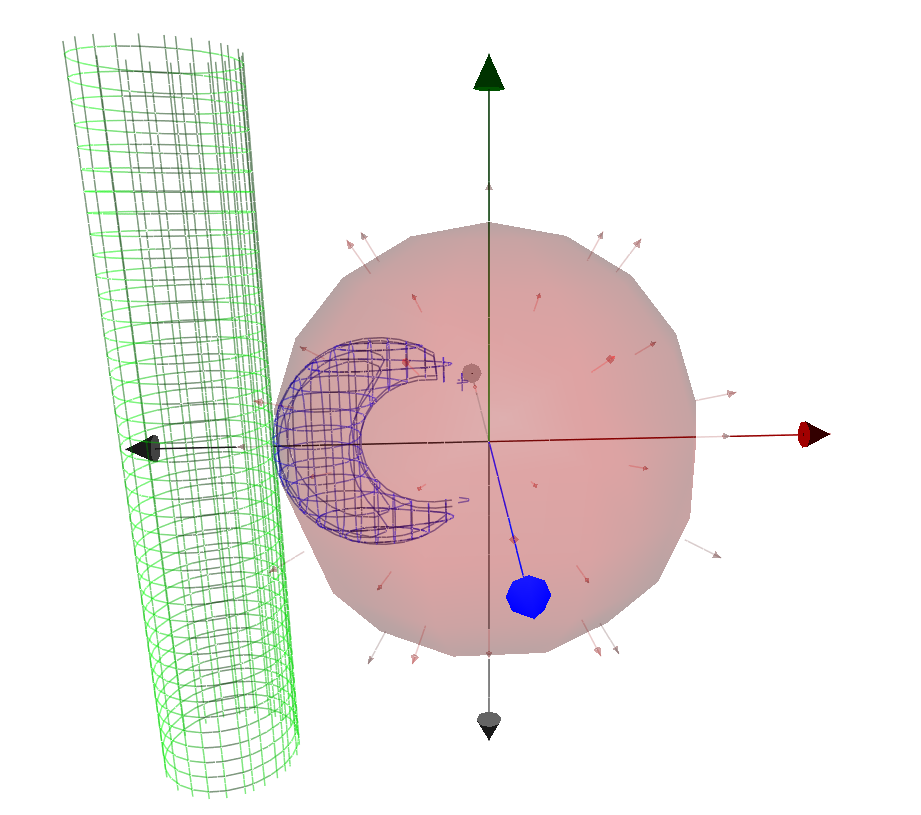
\includegraphics[scale=0.4]{ReflectCylinderInSphere}
\caption{The blue inversion of a green cylinder in a red sphere.  Traces in various planes were
used to render the cylinder and its inversion.}
\label{fig_reflect_cylinder_in_sphere}
\end{figure}
The functions beginning with the word ``bind'' create and bind an entity to the given
element of the geometric algebra that is responsible for interpreting that element
as a surface under Definition~\ref{def_surface} or as a surface under the definition
given by the conformal model.  The computer program can then
use traditional methods to render the surface from the extracted polynomial equation.
For example, the polynomial equation in $x$, $y$ and $z$ for the reflected surface presented
in Figure~\ref{fig_reflect_cylinder_in_sphere} is given by
\begin{equation}
\begin{split}
0 =\;& 28.8x^{2} + 11.2x^{3} + x^{4} + 11.2xy^{2} + 2x^{2}y^{2} + \\
 & 11.2xz^{2} + 2x^{2}z^{2} + y^{4} + 2y^{2}z^{2} + 28.8z^{2} + z^{4}.
\end{split}
\end{equation}
It is interesting how a bit of reasoning in geometric algebra has given us a means
to finding this polynomial equation.
Of course, while such equations lend themselves to computer algorithms, they
are not practical on paper.  This is where the canonical forms of elements may become
useful.

\section{A Companion Algebra $\G([\B(\W)])$ For $\G(\W)$}

In this section we show that there is a geometric algebra where
the $k$-blades of that algebra represent the intersection of $k$ surfaces.\footnote{In
algebraic geometry, these are called algebraic sets or sometimes algebraic varieties.}
The key observation is that $\B(\W)$, (which is what we'll use to denote the set
of all bivectors in $\G(\W)$), is simply a linear space, and we can therefore
explore the geometric algebra, denoted by $\G([\B(\W)])$, that is generated by this linear space.

We begin by introducing $[\cdot]$ as a linear function defined on $\B(\W)$, mapping bivectors
of this space into a vector space that we'll denote by $[\B(\W)]$.  For any pair of linearly
independent vectors $x,y\in\W$, we let $[x\wedge y]$ denote a vector in $[\B(\W)]$.  Being a linear
function, we see that $[\cdot]$ is determined entirely by how it maps a basis for $\B(\W)$.
Furthermore, for any two blades $a,b\in\B(\W)$, we will let
\begin{equation}
[a]\cdot[b] = a\cdot b,
\end{equation}
so that thereby $\G([\B(\W)])$ inherits its signature from $\G(\W)$.  We will
use a bold front for elements of $\G([\B(\W)])$ to set them apart from
elements of $\G(\W)$.

What we see now is that if $\{E_i\}_{i=1}^k$ is a set of $k$ surfaces taken from $\B(\W)$,
then the $k$-blade $\mathbf{E}$, given by
\begin{equation}
\mathbf{E} = \bigwedge_{i=1}^k[E_i],
\end{equation}
is representative of the intersection of these $k$ surfaces as the set
of all points $p\in\V^e$, such that
\begin{equation}\label{equ_dual_surf}
0=[P(p)\wedge\overline{P}(p)]\cdot\mathbf{E},
\end{equation}
provided that $\{[E_i]\}_{i=1}^k$ is a linearly independent set.
We refer to $\mathbf{E}$ here as a dual surface in the case that
we are interpreting it as a surface by equation \eqref{equ_dual_surf}.
If we are interpreting $\mathbf{E}$ as a surface by the equation
\begin{equation}
0=[P(p)\wedge\overline{P}(p)]\wedge\mathbf{E},
\end{equation}
then we refer to $\mathbf{E}$ as a direct surface.  Any blade $\mathbf{E}\in\G([\B(\W)])$
is simultaneously representative of two surfaces, one dually, the other directly.\footnote{It is
sometimes useful to reinterpret a dual geometry as a direct geometry, or vice versa.  For example,
while the outer product of two dual geometries may be a dual imaginary intersection, it may
be a real geometry in direct form.}
It can be shown that a given surface is simultaneously represented by two blades
in $\G([\B(\W)])$ that are duals of one another.

We will now let $\mathbf{I}$ denote, not the psuedo-scalar of $\G([\B(\W)])$, but
the psuedo-scalar of a desired geometric sub-algebra of $\G([\B(\W)])$.  The desired
sub-algebra is generated by the desired sub-space of $[\B(\W)]$.  Our first inclination
might be that this space is the set of vectors
\begin{equation}
\{[x\wedge\overline{y}]:x,y\in\V\},
\end{equation}
which is of dimension $(n+2)^2$, but what we'll find later on is that we want
the dimension of our sub-space to be as small as possible.  To that end,
notice that there
are $n+2$ basis vectors for $\V$ by table \eqref{equ_vector_spaces},
and so to represent a surface $E\in\G(\W)$ by Definition~\ref{def_surface},
we really only need $(n+2)(n+3)/2$ of the $(n+2)^2$ basis 2-blades spanning $\B(\W)$.
We will let $\mathbf{I}$ be
the psuedo-scalar of the geometric sub-algebra of $\G([\B(\W)])$ generated
by this vector sub-space of $[\B(\W)]$ having this irreducible dimension.

To use $\mathbf{I}$ now to take duals of blades $\mathbf{E}\in\G([\B(\W)])$ to
switch between the dual and direct forms, we must restrict our attention
to those surfaces $E\in\G(\W)$ of reduced form.  We will assume this
reduced form from now on.

Before moving on, we should note here that finding the transformation $\mathbf{E}'$ of
a $k$-blade $\mathbf{E}\in\G([\B(\W)])$ by a versor $V\in\G(\V)$ can be done, if
we can find a factorization $\mathbf{E}_1\wedge\dots\wedge\mathbf{E}_k$ of $\mathbf{E}$.
Having such a factorization, we may proceed to write
\begin{equation}
\mathbf{E}' = \bigwedge_{i=1}^k[V\overline{V}[\mathbf{E}_i]^{-1}(V\overline{V})^{-1}].
\end{equation}
The problem of blade factorization was given a great deal of treatment in \cite{}.

\section{Fitting Surfaces To Points}

We have already seen that $\G([\B(\W)])$ can be used to represent
the intersections of surfaces in both direct and dual form, but unlike
the conformal model of geometric algebra, it appears that working
in $\G([\B(\W)])$ is not as practical in the sense that we cannot easily
find canonical forms for certain types of geometries, much less use
them to interpret an intersection result.  Nevertheless, we show
in this section that $\G([\B(\W)])$ does have an interesing application.

Recall that while the outer product of dual geometries can give us a
dual intersection, the outer product of direct geometries can give us
a geometry that is at least the union of the two geometries taken in the product.
One application of this idea is that of fitting a surface to a set of points.

Letting $\{p_i\}_{i=1}^k$ be a set of $k$ points taken from $\V^e$,
we observe that if the corresponding set $\{[P(p_i)\wedge\overline{P}(p_i)]\}_{i=1}^k$
is a linearly independent set, then the elements $\mathbf{E}\in\G([\B(\W)])$, given by
\begin{equation}\label{equ_point_fit}
\mathbf{E} = \bigwedge_{i=1}^k[P(p_i)\wedge\overline{P}(p_i)],
\end{equation}
is directly representative of a surface containing all of these points.  The question
then remains; under what condition on the set of points in $\{p_i\}_{i=1}^k$
is the set $\{[P(p_i)\wedge\overline{P}(p_i)]\}_{i=1}^k$ linearly independent,
and under these circumstances, what surface do we get with $\mathbf{E}$
in equation \eqref{equ_point_fit}?  This question is easy to answer in
the conformal model of geometric algebra, but not so easy here.  No being
able to find an answer, the author is compelled to leave it as an open question.

Another question to consider is that of how many points are needed
to fit a surface of some dimension.  A $k$-blade $\mathbf{E}\in\G([\B(\W)])$
dually represents a surface of dimension $n-k+1$, and therefore,
the blade $\mathbf{EI}$ of grade
\begin{equation}
\mbox{grade}(I)-(n-k+1)
\end{equation}
directly represents
such a surface, which grade is also the number of points we would need
to fit the surface.  Seeing that with the more points we have, the less likely
the set $\{[P(p_i)\wedge\overline{P}(p_i)]\}_{i=1}^k$ is of being linearly independent,
the reader can now see why
we have restricted our attention to only the reduced form of surfaces $E\in\G(\W)$.

\section{Closing Remarks}

If the reader has come this far, then it is likely that he or she has been willing
to forgive the obvious inadequacies of the author; most notably a lack of
awareness of modern day theories of quadratic forms and the entire subject of algebraic
geometry.  (See \cite{} for an in-depth history of quadratic forms.  A history
of algebraic geometry is given with similar uses of strange and foreign terms in \cite{}.)


\nocite{Dorst07}
\bibliographystyle{amsplain}
\bibliography{Parkin_AnExtensionOfTheQuadricModel}

% cite http://www.math.ethz.ch/~knus/papers/campinas.pdf -> quad forms determine clifford algebras?
% cite http://www.maths.ed.ac.uk/~aar/books/dublin.pdf for history of quadratic forms
% cite wiki entry for algebraic variety?

\end{document}